\chapter{Markov Decision Processes}
\label{ch_mdp}

We start by introducing Markov chains, a simpler type of
probabilistic processes which does not offer choices to be made,
then continue to generalize to Markov Decision Processes.
We then overview known approaches to {\em verification} (checking if a
given MDP satisfies a given property) with special focus on Bounded
Real-Time Dynamic Programming which will be used in later chapters.

It is assumed the reader is familiar with basic notions of probability
theory, namely probability function, distribution and random variable.
We use $P(E)$ to denote the probability of an event $E$ and
$\distribution{S}$ to denote the set of probability distributions on a set $S$.

As we work with probabilities over uncountable sets the reader should be
familiar with measure-theoretic treatment of probability (or at least
ready to believe their intuition built with basic probability works here).
Developing the theory here would significantly extend the text while
providing little value so we instead refer the reader to
\parencite{probability}.

\section{Markov Chains}

Markov chain is a simpler formalism than
Markov decision process and provides a good first intuition about
probabilistic models. In a Markov chain there are no decisions, only
probabilities of transition.

\begin{definition}
    Let $S$ be a set of states.
    A sequence of random variables $(X_i)^{\infty}_{i=0}$
    is called a {\em discrete-time Markov chain},
    if the probability of moving to a state is given only by the
    current state, that is
    $P(X_{k+1} = s_{k+1} \mid X_k = s_k) =
    P(X_{k+1} = s_{k+1} \mid X_k = s_k, X_{k-1} = s_{k-1},
    \ldots, X_{1} = s_{1})$ for every $s_j \in S, 1 \leq j \leq k + 1$,
    if the conditional probabilities are defined.
\end{definition}

In many applications it is natural to have an initial state
$s$ ($X_1 = s$) and a chain can
then be drawn as a graph with probabilistic transitions. Note
that the weights of the outgoing edges from a node sum to one, as the
transition probabilities form a distribution on the set of states (for
simplicity we do not draw the transitions with zero probability).

\begin{example}
    \label{ex_mc}
    In this example $s_0$ is the initial state,
    $P(X_2 = s_1 \mid X_1 = s_0) = 0.5$,
    $P(X_2 = s_2 \mid X_1 = s_0) = 0.25$,
    $P(X_2 = s_0 \mid X_1 = s_0) = 0.25$.

\hfill \break
\centering
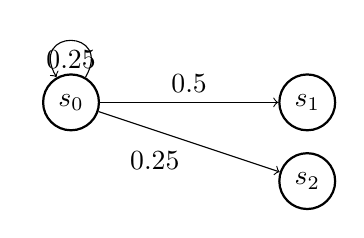
\begin{tikzpicture}
    \tikzstyle{state}=[thick,draw=black,circle]
    \tikzstyle{decision}=[draw,shape=circle,fill=black]

    %\node[state] at (0,0) (s0) {$s_0$};
    %\node[state] at (2,0) (s0b) {};
    %\node[state] at (4,0) (s1) {$s_1$};
    %\node[state] at (4,-1) (s2) {$s_2$};

    %\draw (s0) edge [bend left, ->] node [midway, above] {} (s0b);
    %\draw[->] (s0b) -- (s1) node [midway, above] {0.5};
    %\draw (s0b) edge [bend left, ->] node [midway, below] {0.25} (s0);
    %\draw[->] (s0b) -- (s2) node [midway, below left] {0.25};
    \node[state] at (0,0) (s0) {$s_0$};
    \node[state] at (3,0) (s1) {$s_1$};
    \node[state] at (3,-1) (s2) {$s_2$};

    \draw[->] (s0) -- (s1) node [midway, above] {0.5};
    \draw (s0) edge [->, loop below] node [midway, below] {0.25} (s0);
    \draw[->] (s0) -- (s2) node [midway, below left] {0.25};
\end{tikzpicture}
\end{example}

\begin{example} The Drunkard's Walk is a well known example of a Markov
    chain. One can imagine a drunk person starting in the middle of a road
    (state $s_0$) and then moving randomly left or right. How many times
    will the drunk visit the middle of the road? How many steps will it
    take the drunk on average to reach a ditch ($s_{-2}, s_2$)?

\hfill \break
\centering
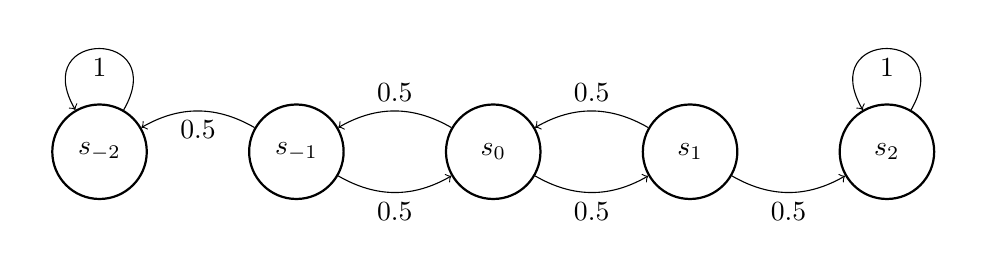
\begin{tikzpicture}
    \tikzstyle{state}=[thick,draw=black,circle, minimum size=1.2cm]
    \tikzstyle{decision}=[draw,shape=circle,fill=black]

    \node[state] at (-5,0) (sm2) {$s_{-2}$};
    \node[state] at (-2.5,0) (sm1) {$s_{-1}$};
    \node[state] at (0,0) (s0) {$s_0$};
    \node[state] at (2.5,0) (s1) {$s_1$};
    \node[state] at (5,0) (s2) {$s_2$};

    \draw (sm2) edge [->, loop below] node [midway, below] {1} (sm2);
    \draw (sm1) edge [->, bend right] node [midway, below] {0.5} (sm2);

    \draw (s0) edge [->, bend right] node [midway, above] {0.5} (sm1);
    \draw (sm1) edge [->, bend right] node [midway, below] {0.5} (s0);

    \draw (s0) edge [->, bend right] node [midway, below] {0.5} (s1);
    \draw (s1) edge [->, bend right] node [midway, above] {0.5} (s0);

    \draw (s1) edge [->, bend right] node [midway, below] {0.5} (s2);
    \draw (s2) edge [->, loop below] node [midway, below] {1} (s2);
\end{tikzpicture}
\end{example}

\section{Markov Decision Processes}

Markov decison processes are similar to Markov chains, except now an
actor interacting with the process can in each state pick an action
and the next state is chosen according to a distribution on states
corresponding to this action.

\begin{definition}
A {\em Markov Decision Process} is a tuple $(S, A, E, \Delta)$, where
$S$ is a finite set of states,
%$s \in S$ is the initial state,
$A$ is a finite set of actions,
$E : S \to \powerset{A}$ gives the set of enabled actions in a state,
and $\Delta : S \times A \to \distribution{S}$ is a partial transition
function which assigns a probability distrubution on states to an action
and a state.

It is assumed without loss of generality that for all $s \neq s'$ it
holds that $E(s) \cap E(s') = \emptyset$. If this didn't hold the
actions could just be renamed.
\end{definition}

\begin{example}
    \label{ex_mdp}
    The MDP $(\{s_0, s_1, s_2\}, \{a\}, E, \Delta)$,
    where
    $E(s_0) = \{a,b\}$, $E(s_1) = E(s_2) = \emptyset$,
    and $\Delta(s_0, a) = \{(s_1, 1)\}$,
    $\Delta(s_0, b) = \{(s_1, 0.5),$ $(s_2,0.25), (s_0,0.25)\}$
    is depicted below.
    The edges labeled with letters denote the available actions
    and lead to smaller black dots, which mark the point of random
    choice of the successor state.

    The actor making decisions should choose action $a$ if
    they want to get to $s_1$, or (possibly repeatedly) choose $b$ if
    they want to get to $s_2$ (the achievement of this goal is not
    guaranteed).

\hfill \break
\centering
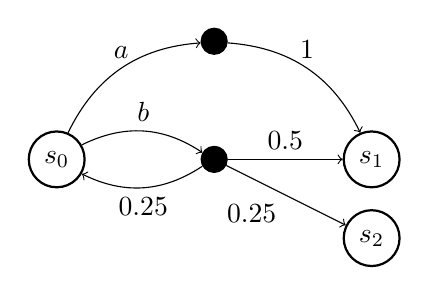
\begin{tikzpicture}
    \tikzstyle{state}=[thick,draw=black,circle]
    \tikzstyle{transition}=[draw,shape=circle,fill=black]

    \node[state] at (0,0) (s0) {$s_0$};
    \node[transition] at (2,1.5) (s0a) {};
    \node[transition] at (2,0) (s0b) {};
    \node[state] at (4,0) (s1) {$s_1$};
    \node[state] at (4,-1) (s2) {$s_2$};

    \draw (s0) edge [bend left, ->] node [midway, above] {$a$} (s0a);
    \draw (s0a) edge [bend left, ->] node [midway, above] {$1$} (s1);
    \draw (s0) edge [bend left, ->] node [midway, above] {$b$} (s0b);
    \draw[->] (s0b) -- (s1) node [midway, above] {0.5};
    \draw (s0b) edge [bend left, ->] node [midway, below] {0.25} (s0);
    \draw[->] (s0b) -- (s2) node [midway, below left] {0.25};
\end{tikzpicture}

\end{example}

A standard use of Markov decision processes has been in areas where it
is useful to operate with rewards. This definition will be useful later.

\begin{definition}
If $(S, A, E, \Delta)$ is a Markov decision process,
%$a \in A, s, s' \in S$, $a \in E(s)$, $\Delta(s,a)(s') > 0$,
and $R : S \times A \times S \to \mathbb{R}$ is a function,
then $(S,A,E,\Delta,R)$ is a {\em Markov decision process with rewards}.
\end{definition}


\begin{definition}[Path]
    An {\em infinite path} is
    a sequence $\omega = s_0 a_0 s_1 a_1
    \ldots$ such that $a_i \in E(s_i)$ for all $i \in \mathbb{N}$.
    The set of all infinite paths of is denoted $IPaths$.

    A {\em finite path} is a prefix of an infinite path such that it
    ends with a state. The last state for a finite path $\rho$ is
    denoted $\last(\rho)$. The set of all finite paths is denoted
    $FPaths$.
\end{definition}

When following a path one wants to avoid getting stuck in
an infinitely repeated cycle of states and actions. The parts of MDP
where this happens are called end components.
An example end component is shown in \autoref{fig:non-triv-ec}.

\begin{definition}[End component]
Let $\mathcal{M} = (S, A, E, \Delta)$ be an MDP,
let $S' \subseteq S$ and $A' \subseteq \bigcup_{s' \in S'} E(s')$.
The pair $(S', A')$ is an {\em end component},
if for every $s \in S', s' \in S, a \in A'$ it holds that
$\Delta(s,a)(s') > 0 \implies s' \in S'$,
and if there is a path between every two $s, s' \in S'$
using only actions in $A'$.
\end{definition}

TODO: potrebujeme definovat maximal end component? Pokud ano, tak staci
zminit, ze jako usporadani uvazujeme mnozinove usporadani po slozkach.

\begin{figure}[ht]
\begin{center}
\begin{tikzpicture}
    \tikzstyle{state}=[thick,draw=black,circle]
    \tikzstyle{transition}=[draw,shape=circle,fill=black]

    \draw[<-] (s0) -- node[above] {} ++(-1cm,0);

    \node[state] at (0,0) (s0) {$s_0$};
    \node[state] at (2,0) (s1) {$s_1$};
    \node[state] at (4,0) (s2) {$s_2$};

    \draw (s0) edge [bend left, ->] node [midway, above] {$a$} (s1);
    \draw (s1) edge [bend left, ->] node [midway, below] {$b$} (s0);
    \draw (s1) edge [->] node [midway, above] {$c$} (s2);
\end{tikzpicture}
\end{center}
\caption{An MDP with a non-trivial end component.}
\label{fig:non-triv-ec}
\end{figure}

The following definition introduces what is commonly called strategy,
policy, scheduler, controller or adversary. It is the decision maker in
the MDP which looks at the path traversed so far and assigns each action
$a$ in the last (current) state the probability of $a$ being chosen.

\begin{definition}[Strategy]
    Let $\mathcal{M} = (S,A,E,\Delta)$ be a Markov decision process
    and $\rho \in FPaths$.
    A {\em strategy} is a function
    $\sigma : FPath \to Dist(A)$
    such that\footnote{
The condition ensures that only actions which can
be chosen have non-zero probability assigned by the strategy.
    }
    $\sigma(\rho)(a) > 0 \implies a \in E(\last(\rho))$.

    A strategy $\sigma$ is {\em memoryless} if $\sigma(\rho)$ depends
    only on $\last(\rho)$.
\end{definition}

What happens once the strategy is fixed? The MDP becomes a Markov chain.
This can be seen in the examples, e.g. if the strategy is to always
choose $b$, the MDP from \autoref{ex_mdp} becomes the MC from
\autoref{ex_mc}.

For very small MDPs this gives the first algorithm for evaluating their
properties: for every strategy reduce the MDP to a Markov chain and evaluate the
property using known Markov chain algorithms, then aggregate the
results\footnote{The idea of this naive method can be significantly improved and instead
of exploring a vast amount of strategies only a small portion of
reasonably good strategies is explored \parencite{smc}.}.


% http://www.lsv.fr/axes/VASCO/gdt/haddad_gdt_20012016.pdf

\noindent {\bf Observability of MDP.}
One can distinguish between various levels of knowledge about an MDP,
usually depending on the source of the model.
In partially observable MDPs the information about $\Delta$ may not be
available (but algorithms for solving the reachability
problem in such MDPs exist too \parencite{atva14}). This thesis deals
only with fully observable MDPs.


\section{Verification}

{\em Formal verification} is the act of proving that a given system satisfies
a given property. {\em Model
checking} is an approach to formal verification which uses a model of
the system to verify the property.

In our case the systems are modelled as Markov decision processes and
the properties are concerned about maximum probability of reaching a state.

\noindent \textbf{Reachability probability.}

$P^\sigma_{\mathcal{M},s}(\lozenge F)$

Importantly there is always a memoryless strategy maximizing the
reachability probability. Puterman \parencite{puterman} proves this for
reward maximization and we can use his proof with a simple reduction.
For any MDP create an MDP with rewards, such that the reward function
is zero everywhere, except when entering a target state it gives reward 1
and when leaving a target state it gives reward -1. TODO: Check this is
right.

A description of the most common approaches to computing Pr... follows.
Standard algorithms Value Iteration and Strategy Iteration are shown
and later we describe BRTDP.

One approach we do not explain is formulating the problem as a system
linear equations and solving it. The solution is precise and has
guaranteed correctness but the computation quickly becomes expensive as
the model grows in size.  See \parencite{forejt} for a description of
this method.

\subsection{Value Iteration}

Value iteration (in its variation for computing expected maximum rewards) is a
dynamic programming algorithm which was first described by Richard
Bellman (known for introducing the term dynamic programming) in 1957
\parencite{bellman}.

Before showing the algorithm we first note that it will need to
process all states. However, the values in some states are quite easy to
compute and a preprocessing will allow for reduction of the
state space.

These easy states are in set $Z$
of {\em zero states} or set $F'$ of {\em extended target states}
for given MDP $\mathcal{M}$. These are states $z
\in Z$ such that for any $\sigma \in \Sigma$ it holds that
$P^\sigma_{\mathcal{M},z}(\lozenge F) = 0$,
and $f \in F$ such that ... TODO.

The main idea of value iteration is materialized in the following
recurrence relation for newly introduced variables $x_s^n, s \in S, n
\in \mathbb{N}$.
\[
x_s^n =
\begin{cases}
    1 & \text{if }s \in F \cup F' \\
    0 & \text{if }s \in Z \lor (s \not \in F \land n = 0) \\
    \max\limits_{a \in E(s)} \sum\limits_{s' \in S} \Delta(s,a)(s') \cdot x_{s'}^{n-1}
    & \text{otherwise} % \text{if }s \in S \setminus (F \cup Z)
\end{cases}
\]
By computing $x^n$ for $n = 1,2,\ldots$ we gain increasingly precise
estimate of the actual maximum reachability probability,
formally $\lim_{n \to \infty} x^n_s = P_{\mathcal{M},s}(\lozenge F)$.
TODO: prove (use Puterman's proof with reward $1$ when reaching target
state, 0 otherwise).

This recurrence relation is now turned into a dynamic programming
algorithm as shown in \autoref{vi}. Instead of iterating $n$ times the
algorithm proceeds with its computations while the convergence is not
slow (the threshold is given by some $\epsilon$). Limit on the number of
iterations may be introduced if we want to check time bounded
properties.

\begin{algorithm}
\caption{Value Iteration}
\label{vi}
\begin{algorithmic}
    \State $\forall s \in S,\; s \gets$ if $x \in F$ then $1$ else $0$
    \Do
        \ForEach{$s \in S \setminus (F \cup Z)$}
            \State $x_s \coloneqq
            \max_{a \in E(s)} \sum_{s' \in S} \Delta(s,a)(s') \cdot x_{s'}$
        \EndFor
    \doWhile{the change of $x_s$ for any $s$ is greater than $\epsilon$}
\end{algorithmic}
\end{algorithm}

Value iteration is an easy method for computing the reachability
probability of a given MDP.  However we only have a proof of convergence
and not a good stopping criterion.  Furthermore it is doing extra work
on models where only a small part needs to be explored to find a good
strategy as it has to compute its results for all the states.

The solution to the first issue is the {\em interval iteration}
algorithm \parencite{interval_iteration}, an algorithm in parts similar
to value iteration but which maintains lower and upper bounds of the
sought probability. The algorithm has a well-defined stopping criterion
and a bound on the running time.  We will explore solutions to the
second issue later with heuristic methods.

% http://www.sciencedirect.com/science/article/pii/S0304397516307095
% http://pageperso.lif.univ-mrs.fr/~benjamin.monmege/talks/MoVe2015.pdf

\subsection{Strategy Iteration}

Strategy Iteration (also Policy Iteration).
Describe origin
How it works
Pros and cons

\section{Bounded Real-Time Dynamic Programming}

When only a portion of an MDP needs to be searched to find the right
strategy there is an opportunity to employ algorithms which avoid
searching the whole state space. Bounded Real-Time Dynamic Programming
(BRTDP) is such an algorithm. Originally developed for
the objective of finding the best-profit strategy
\parencite{profit_brtdp} the algorithm was adapted to the problem of
verification \parencite{atva14}.

Let us define the {\em value function} $V : S \times A \to
[0,1]$ for all $s \in S, a \in E(s)$ as follows

\[
    V(s,a) \coloneqq \sum_{s' \in S} \Delta(s,a)(s')V(s')
\]
(TODO: Define $\mathcal{M}$ which is used further)
BRTDP is learning $V$ by computing its lower and upper bounds $L, U$
through simulated runs of $\mathcal{M}$ from the given initial state.
TODO: CONTINUE explanation
TODO: Assume no MECs besides trivial

\begin{algorithm}
\caption{BRTDP for MDPs without end components}
\label{brtdp}
\begin{algorithmic}
\State $U(s,a) \gets 1, L(s,a) \gets 1 \; \forall s \in S, a \in E(s)$
\State $U(z,a) \gets 0, L(t,a') \gets 1
    \; \forall z \in zero states, a \in E(z)
    \; \forall t \in target states, a' \in E(t)$
\State $s \gets s_0$
\While{max diff in initial is greater than epsilon}
    % explore
    \State \# Explore Phase
    \While{$s \not \in target \cup zero$}
        \State $a \gets$ sample uniformly from
        \State $s \gets $ sample according
        \State $\omega \gets \omega \; a \; s$
    \EndWhile

    % update
    \State \# Update Phase
    \While{$s \neq s_0$}
        \State $pop(\omega)$
        \State $a \gets pop(\omega)$
        \State $s \gets last(\omega)$
        \State $U(s,a) \coloneqq \sum_{s' \in S} \Delta(s,a)(s')U(s')$
        \State $L(s,a)\, \coloneqq \sum_{s' \in S} \Delta(s,a)(s')L(s')$
    \EndWhile
\EndWhile
\State \Return Action from $v_0$ to the best node (by some
given metric).
\end{algorithmic}
\end{algorithm}

TODO: Prove AC?

\subsection*{BRTDP for MDPs with End Components}
Unfortunately BRTDP is not guaranteed to converge when the MDP
contains non-trivial end components.

\begin{example}
TODO: Describe why BRTDP is stuck here.

\begin{center}
\begin{tikzpicture}
    \tikzstyle{state}=[thick,draw=black,circle]
    \tikzstyle{transition}=[draw,shape=circle,fill=black]

    \draw[<-] (s0) -- node[above] {} ++(-1cm,0);

    \node[state] at (0,0) (s0) {$s_0$};
    \node[state] at (2,0) (s1) {$s_1$};
    \node[transition] at (4,0) (s0b) {};
    \node[state] at (6,-0.7) (s2) {$s_2$};
    \node[state] at (6, 0.7) (s3) {$s_3$};

    \draw (s0) edge [bend left, ->] node [midway, above] {$a$} (s1);
    \draw (s1) edge [bend left, ->] node [midway, below] {$b$} (s0);
    \draw (s1) edge [->] node [midway, above] {$c$} (s0b);

    \draw[->] (s0b) -- (s2) node [midway, below] {0.5};
    \draw[->] (s0b) -- (s3) node [midway, above] {0.5};
\end{tikzpicture}
\end{center}
\end{example}

TODO: Briefly explain how the algorithms gets modified to handle end
components, but not much details and no proofs.

\subsection*{Variants of BRTDP}
When in state $s$ and chosen action $a$,
the choice of the next state does not necessarily have to be done by
sampling the transition distribution $\Delta(s,a)$ (we call this variant
HIGH-PROB) but can be instead be chosen with probability
$\Delta(s,a)(s') \cdot (U(s') - L(s'))$, we call this variant MAX-DIFF.
One can think of other variants, for example round-robin choice.

\begin{example}
\label{brtdp_adversary}
We conclude with an example MDP, which is hard for most variants of BRTDP.
For example the HIGH-PROB TODO

\begin{center}
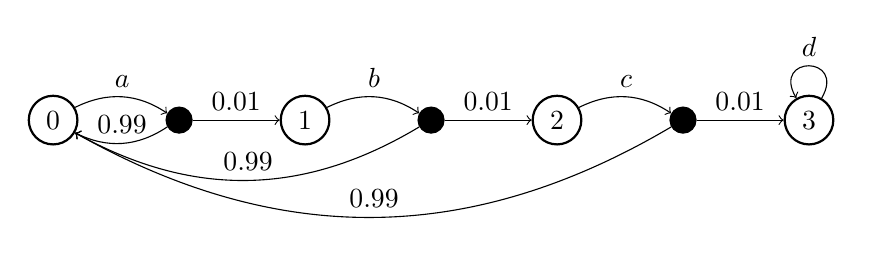
\begin{tikzpicture}
    \tikzstyle{state}=[thick,draw=black,circle]
    \tikzstyle{transition}=[draw,shape=circle,fill=black]
    \tikzstyle{loop}=[looseness=5, in=120, out=60]

    \node[state] at (0,0) (s0) {0};
    \node[transition] at (1.6,0) (s0b) {};
    \node[state] at (3.2,0) (s1) {1};
    \node[transition] at (4.8,0) (s1b) {};
    \node[state] at (6.4,0) (s2) {2};
    \node[transition] at (8,0) (s2b) {};
    \node[state] at (9.6,0) (s3) {3};

    \draw (s0) edge [bend left, ->] node [midway, above] {$a$} (s0b);
    \draw[->] (s0b) -- (s1) node [midway, above] {0.01};
    \draw (s0b) edge [bend left, ->] node [midway, above] {0.99} (s0);

    \draw (s1) edge [bend left, ->] node [midway, above] {$b$} (s1b);
    \draw[->] (s1b) -- (s2) node [midway, above] {0.01};
    \draw (s1b) edge [bend left, ->] node [midway, above] {0.99} (s0);

    \draw (s2) edge [bend left, ->] node [midway, above] {$c$} (s2b);
    \draw[->] (s2b) -- (s3) node [midway, above] {0.01};
    \draw (s2b) edge [bend left, ->] node [midway, above] {0.99} (s0);

    \draw (s3) edge [loop,->] node [above] {$d$} (s3);
\end{tikzpicture}
\end{center}
\end{example}
